\chapter{Технологическая часть}

\section{Выбор операционной системы}

Согласно требованиям технического задания, разрабатываемый портал должен обладать высокой доступностью, работать на типичных архитектурах ЭВМ (Intel x86, Intel x64), а так же быть экономически недорогим для сопровождения. Таким образом, требования к ОС следующие.
\begin{itemize}
	\item \textbf{Распространенность}. На рынке труда должно быть много специалистов, способных администрировать распределенную систему, работающую под управлением выбранной операционной системы.
	\item \textbf{Надежность}. Операционная система должна широко использоваться в стабильных проектах, таких как Mail.Ru, Vk.com, Google.com. Эти компании обеспечивают высокую работоспособность своих сервисов, и на их опыт можно положиться.
	\item \textbf{Наличие требуемого программного обеспечения}. Выбор операционной системы не должен ограничивать разработчиков в выборе программного обеспечения, библиотек.
	\item \textbf{Цена}.
\end{itemize}
 
Под данные требования лучше всего подходит ОС Linux, дистрибутив Ubuntu. \textbf{Ubuntu} \cite{ubuntu} — это дистрибутив, использующий ядро Linux. Как и все дистрибутивы Linux, Ubuntu является ОС с открытым исходным кодом, бесплатным для использования. Поставляется как в клиентской (с графическим интерфейсом), так и в серверной (без графического интерфейса) версиями. Ubuntu поставляется с современными версиями ПО. Преимуществом Ubuntu являются низкие требования к квалификации системных администраторов. Однако Ubuntu менее стабильна в работе.


\section{Выбор СУБД}

В качестве СУБД была выбрана \textbf{PostgreSQL} \cite{postgresql}, так как она наилучшим
образом подходит под требования разрабатываемой системы:
\begin{itemize}
	\item Масштабируемость: PostgreSQL поддерживает горизонтальное масштабирование, что позволяет распределить данные и запросы между несколькими узлами базы данных. Это особенно полезно в географически распределенных системах, где данные и пользователи могут быть разбросаны по разным регионам.
	\item Географическая репликация: PostgreSQL предоставляет возможность
настройки репликации данных между различными узлами базы данных, расположенными в разных географических зонах. Это позволяет
обеспечить отказоустойчивость и более быстрый доступ к данным для
пользователей из разных частей нашей страны.
	\item Гибкость и функциональность: PostgreSQL обладает широким набором
функций и возможностей, что делает его подходящим для различных
типов приложений и использования в распределенной среде. Он поддерживает сложные запросы, транзакции, хранимые процедуры и многое
другое.
	\item Надежность и отказоустойчивость: PostgreSQL известен своей надежностью и стабильностью работы. В распределенной географической
системе это особенно важно, поскольку он способен обеспечить сохранность данных и доступность даже при сбоях в отдельных узлах.
\end{itemize}


\section{Выбор языка разработки и фреймворков компонент
портала}

Для разработки бэкенда существует множество языков программирования, каждый из которых имеет свои сильные и слабые стороны, для данного приложения был выбран \textbf{Python} \cite{python} по следующим причинам:

\begin{enumerate}
	\item Простота и скорость разработки: Python позволяет разработчикам писать меньше кода и быстрее реализовывать функциональность, благодаря удобному синтаксису и мощным фреймворкам (Django, Flask, FastAPI). Это особенно важно для стартапов и небольших проектов, где критично быстрое создание прототипов и внедрение изменений.
	\item Широкая экосистема: В Python существует множество готовых библиотек для работы с базами данных, аутентификацией, кэшированием, очередями, обработкой данных и другими задачами бэкенда. Это ускоряет разработку и снижает количество ручной работы.
	\item Поддержка современных технологий: Python активно используется для задач, связанных с машинным обучением, обработкой данных и научными вычислениями. Это делает его выбором номер один для компаний, работающих с большими данными или развивающих искусственный интеллект.
	\item Сообщество и поддержка: Python имеет одно из крупнейших сообществ разработчиков, что упрощает решение проблем, обновление знаний и получение поддержки.
	\item Универсальность: Python может использоваться не только для разработки веб-приложений, но и для автоматизации, обработки данных и других областей, что делает его многофункциональным инструментом.
\end{enumerate}

В качестве фреймворка для создания веб-приложений на Python был выбран \textbf{FastAPI} \cite{fastapi} по следующим причинам.

\begin{enumerate}
	\item Производительность: FastAPI предлагает одну из самых высоких производительностей среди Python-фреймворков. Это особенно важно для приложений, требующих быстрого отклика при большом количестве запросов, таких как API и микросервисы.
	\item Поддержка асинхронности: В отличие от Django, который частично поддерживает асинхронные операции, FastAPI изначально построен с учетом асинхронного программирования. Это делает его идеальным для приложений, где необходимо эффективно обрабатывать большое количество параллельных запросов (например, в реальном времени или при работе с внешними API).
	\item Простота и автоматическая валидация: FastAPI использует аннотации типов Python для автоматической валидации данных и генерации документации, что значительно упрощает работу с API. Это улучшает качество кода и сокращает количество ошибок.
	\item Генерация документации <<из коробки>>: FastAPI автоматически создает документацию API с использованием стандартов OpenAPI и Swagger. Это экономит время разработчиков и упрощает работу с клиентами и другими командами.
	\item Гибкость и современность: FastAPI предлагает более гибкий и легкий подход к разработке по сравнению с Django, сохраняя простоту и читабельность кода, как в Flask. Он идеально подходит для создания быстрых, масштабируемых и легких приложений, особенно в микросервисной архитектуре.
\end{enumerate}


\section{Выбор фреймворка фронтенд разработки}

Для разработки фронтенда был выбран фреймворк \textbf{React} \cite{react} по следующим причинам.

\begin{enumerate}
	\item Популярность и поддержка сообщества: React является одним из самых популярных инструментов для фронтенд-разработки. Благодаря этому для React доступно множество библиотек, инструментов и ресурсов. Это значительно упрощает разработку, особенно при необходимости интеграции с другими технологиями.
	\item Гибкость: В отличие от Angular, который является <<жестким>> фреймворком с предустановленными решениями, React предлагает больше свободы. Разработчики могут выбирать любые библиотеки для маршрутизации, управления состоянием и работы с сервером, адаптируя проект под конкретные требования.
	\item Производительность через Virtual DOM: React использует Virtual DOM для минимизации реальных изменений в DOM, что делает его быстрым даже для сложных пользовательских интерфейсов. Это особенно важно для крупных приложений с динамически изменяющимися данными.
	\item Поддержка мобильной разработки: React Native предоставляет возможность использовать знания и компоненты React для разработки мобильных приложений под iOS и Android. Это позволяет создавать кроссплатформенные приложения с минимальными усилиями.
\end{enumerate}


\section{Высокоуровневый дизайн пользовательского интерфейса}

Пользовательский интерфейс в разрабатываемой системе представляет собой web-интерфейс, доступ к которому осуществляется через браузер (тонкий клиент). Страница системы состоит из <<шапки>>, бокового меню и основной части.  

Обобщенно структуру страниц системы можно представить следующим образом:
\begin{itemize}
  \item страница авторизации;
	\item страница регистрации;
	\item страница со списком полетов;
	\item страница со списком купленных и сданных билетах;
	\item страница с информацией о пользователе и историей покупок билетов;
	\item страница со статистикой сервиса-координатора.
\end{itemize}

Данные страницы представленны на рисунках \ref{fig:page-01}-\ref{fig:page-07} приведены примеры описанных страниц.

\begin{figure}[H]
	\begin{center}
		{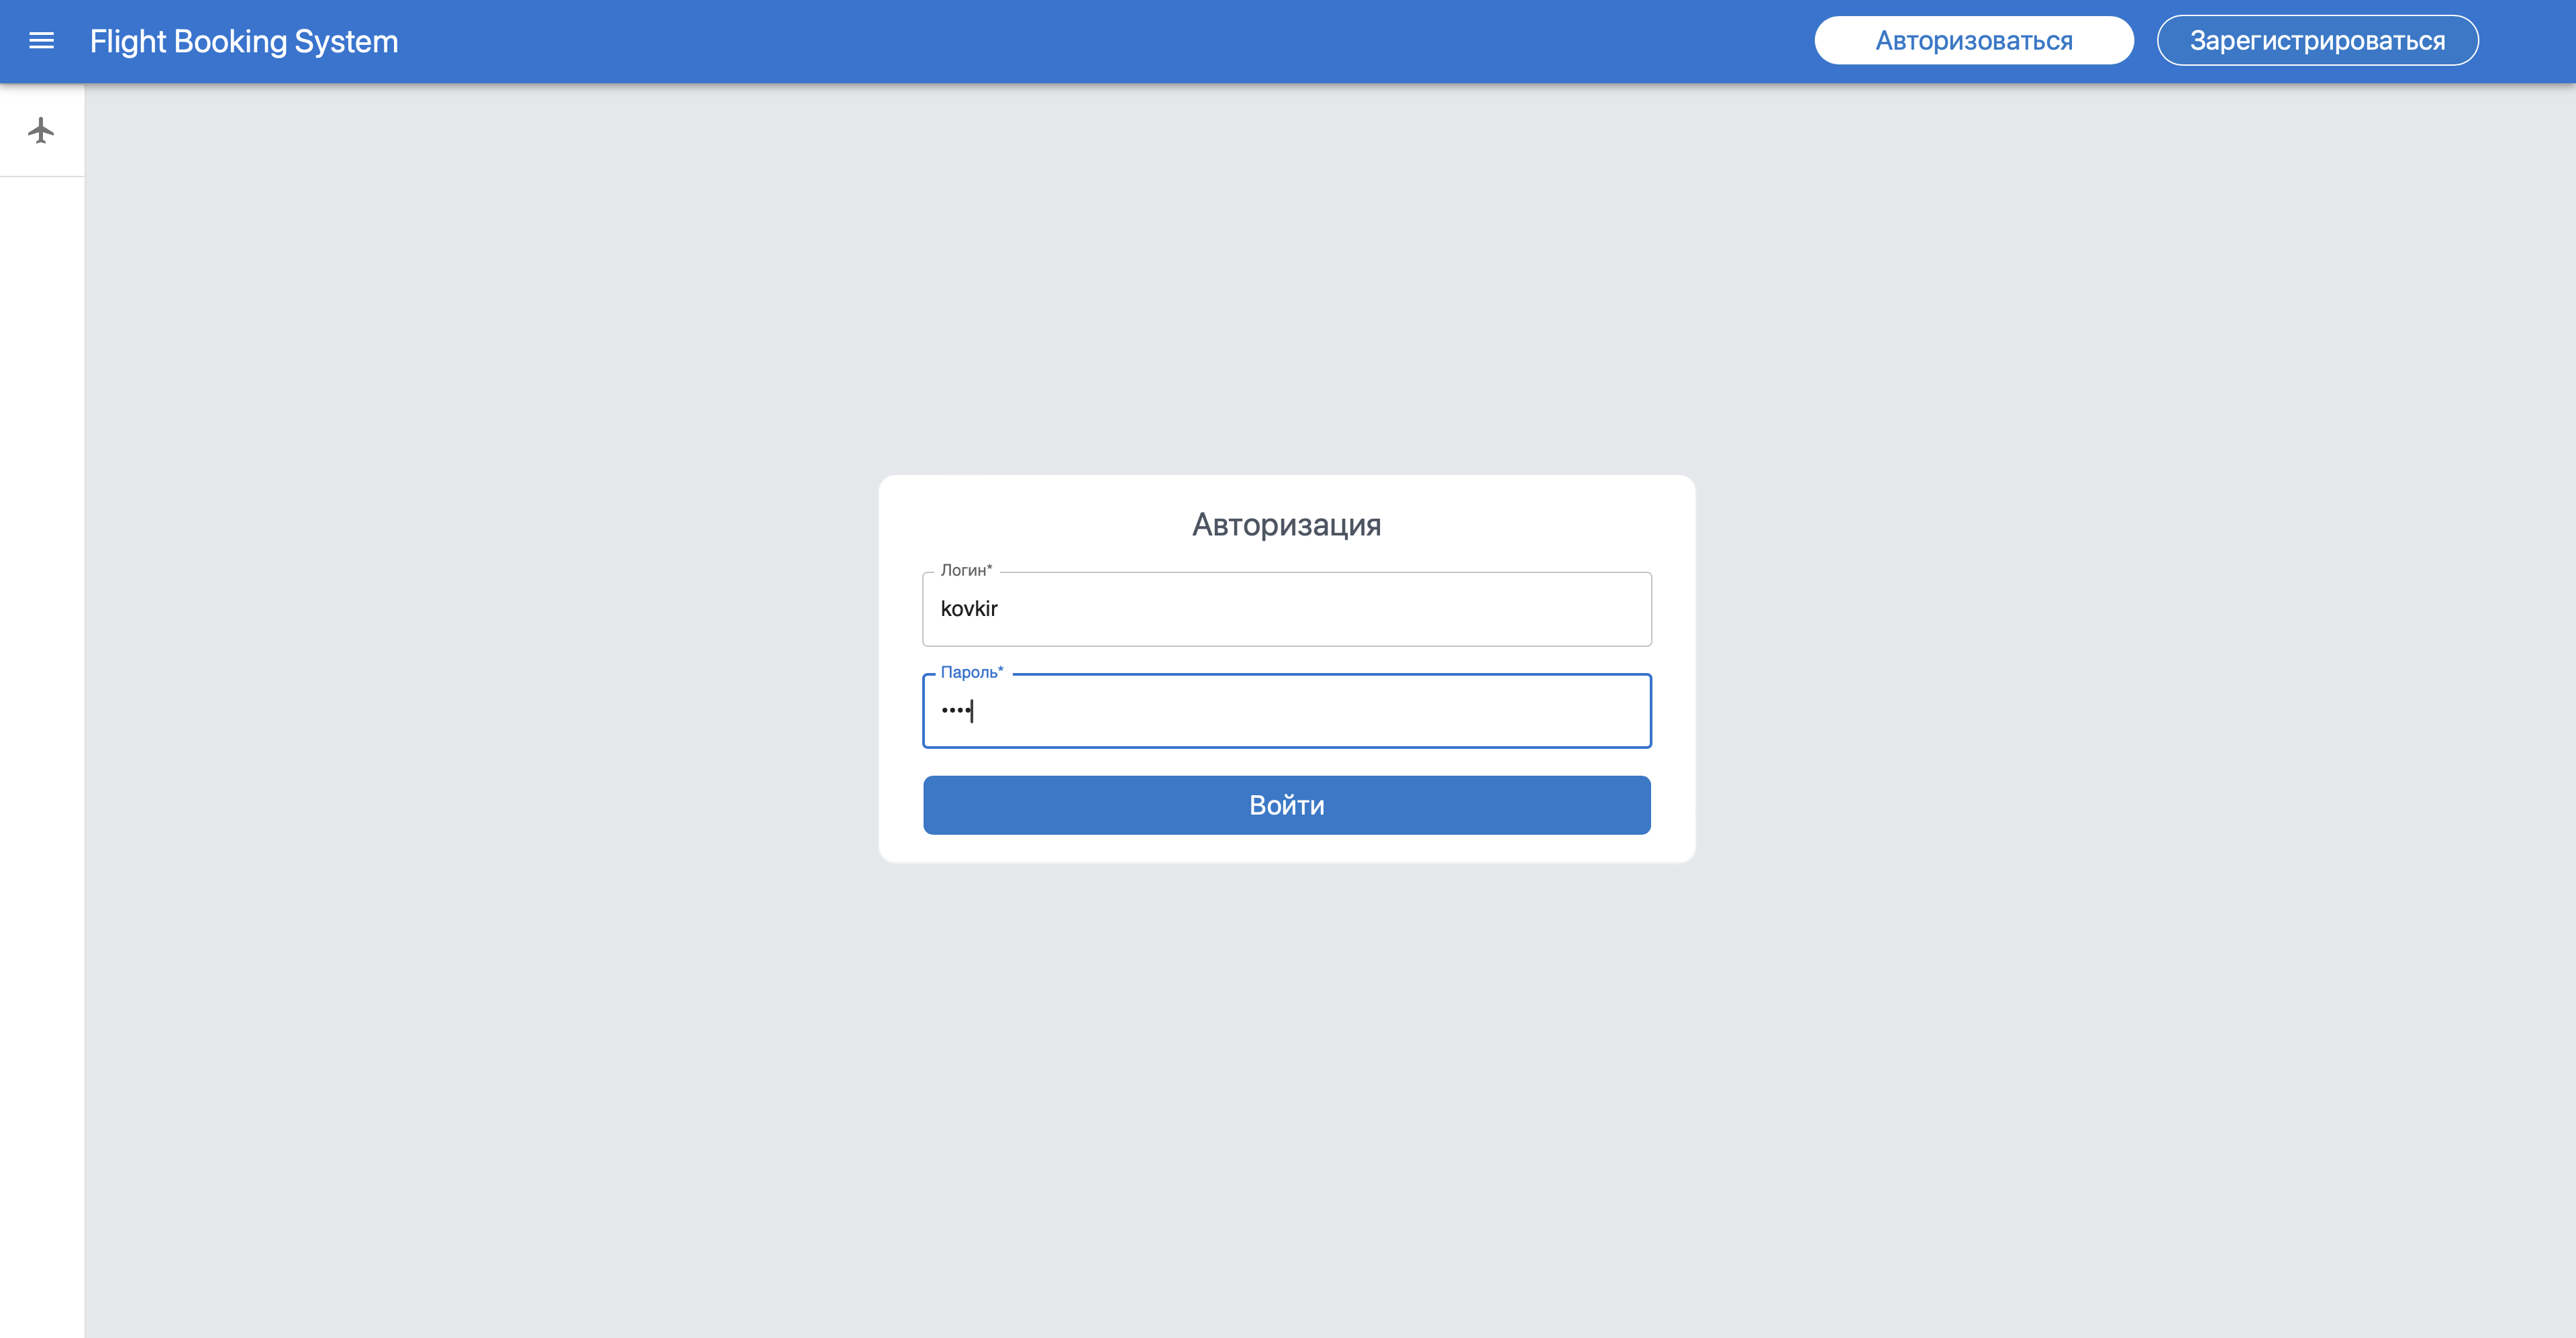
\includegraphics[scale = 0.25]{../img/pages/page-01.png}}
		\caption{Страница авторизации}
		\label{fig:page-01}
	\end{center}
\end{figure}

\begin{figure}[H]
	\begin{center}
		{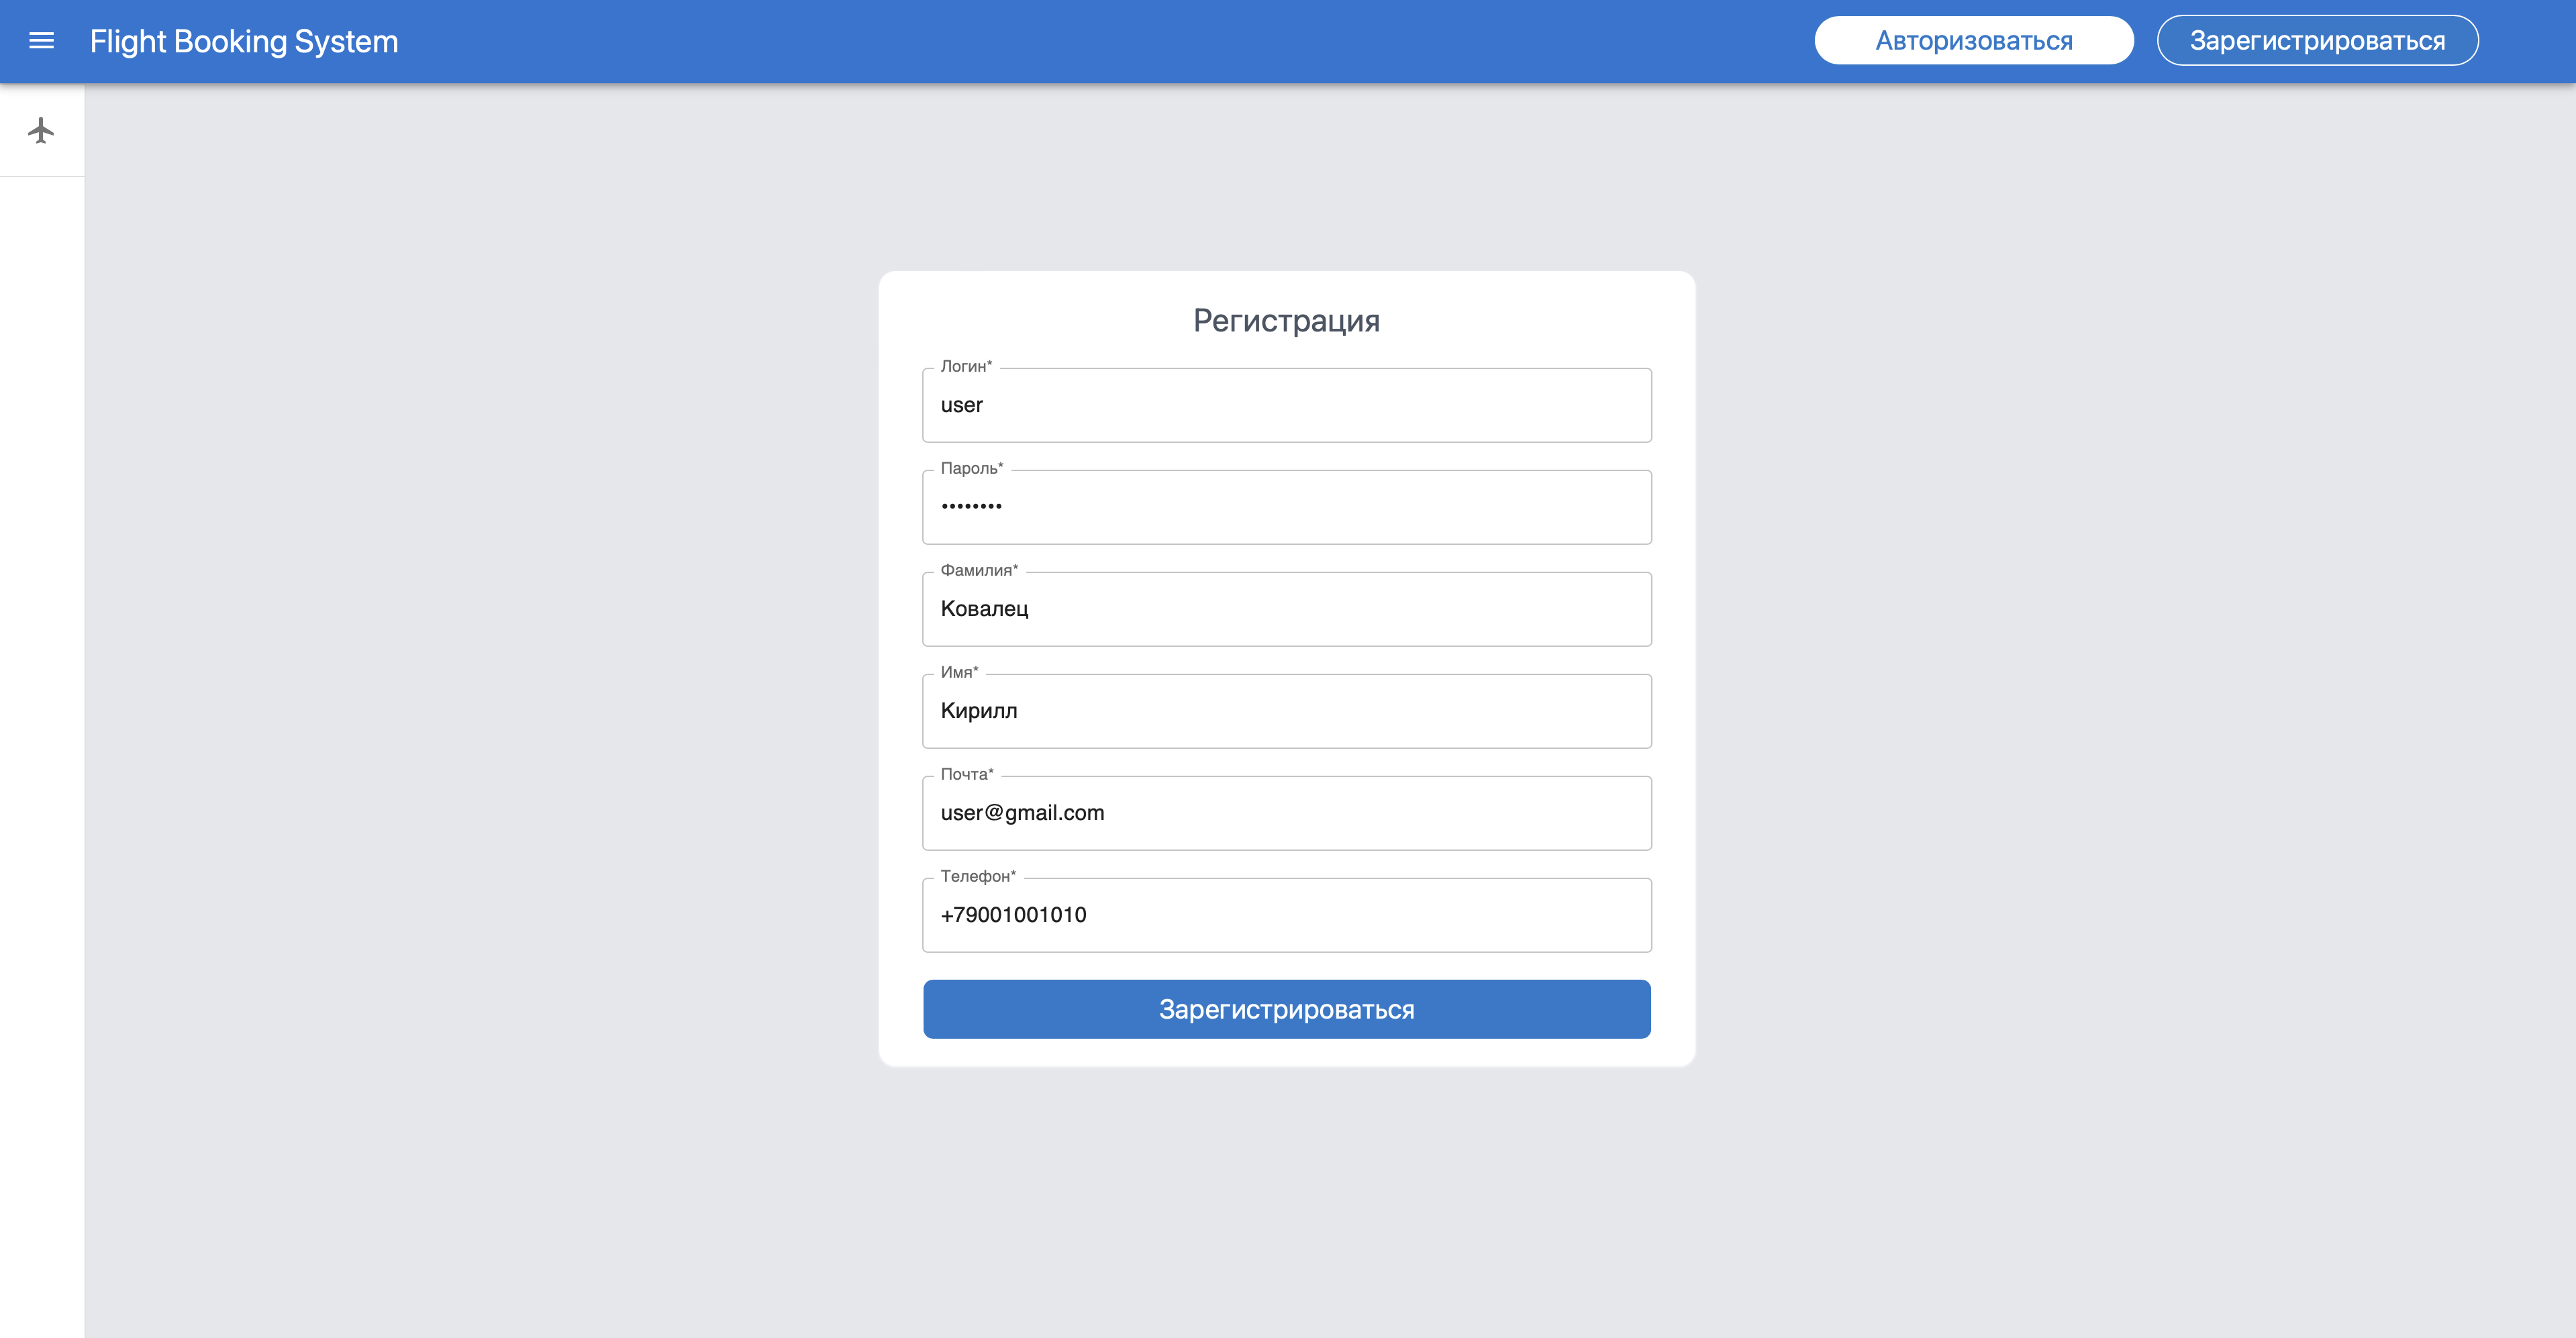
\includegraphics[scale = 0.25]{../img/pages/page-02.png}}
		\caption{Страница регистрации}
		\label{fig:page-02}
	\end{center}
\end{figure}

\begin{figure}[H]
	\begin{center}
		{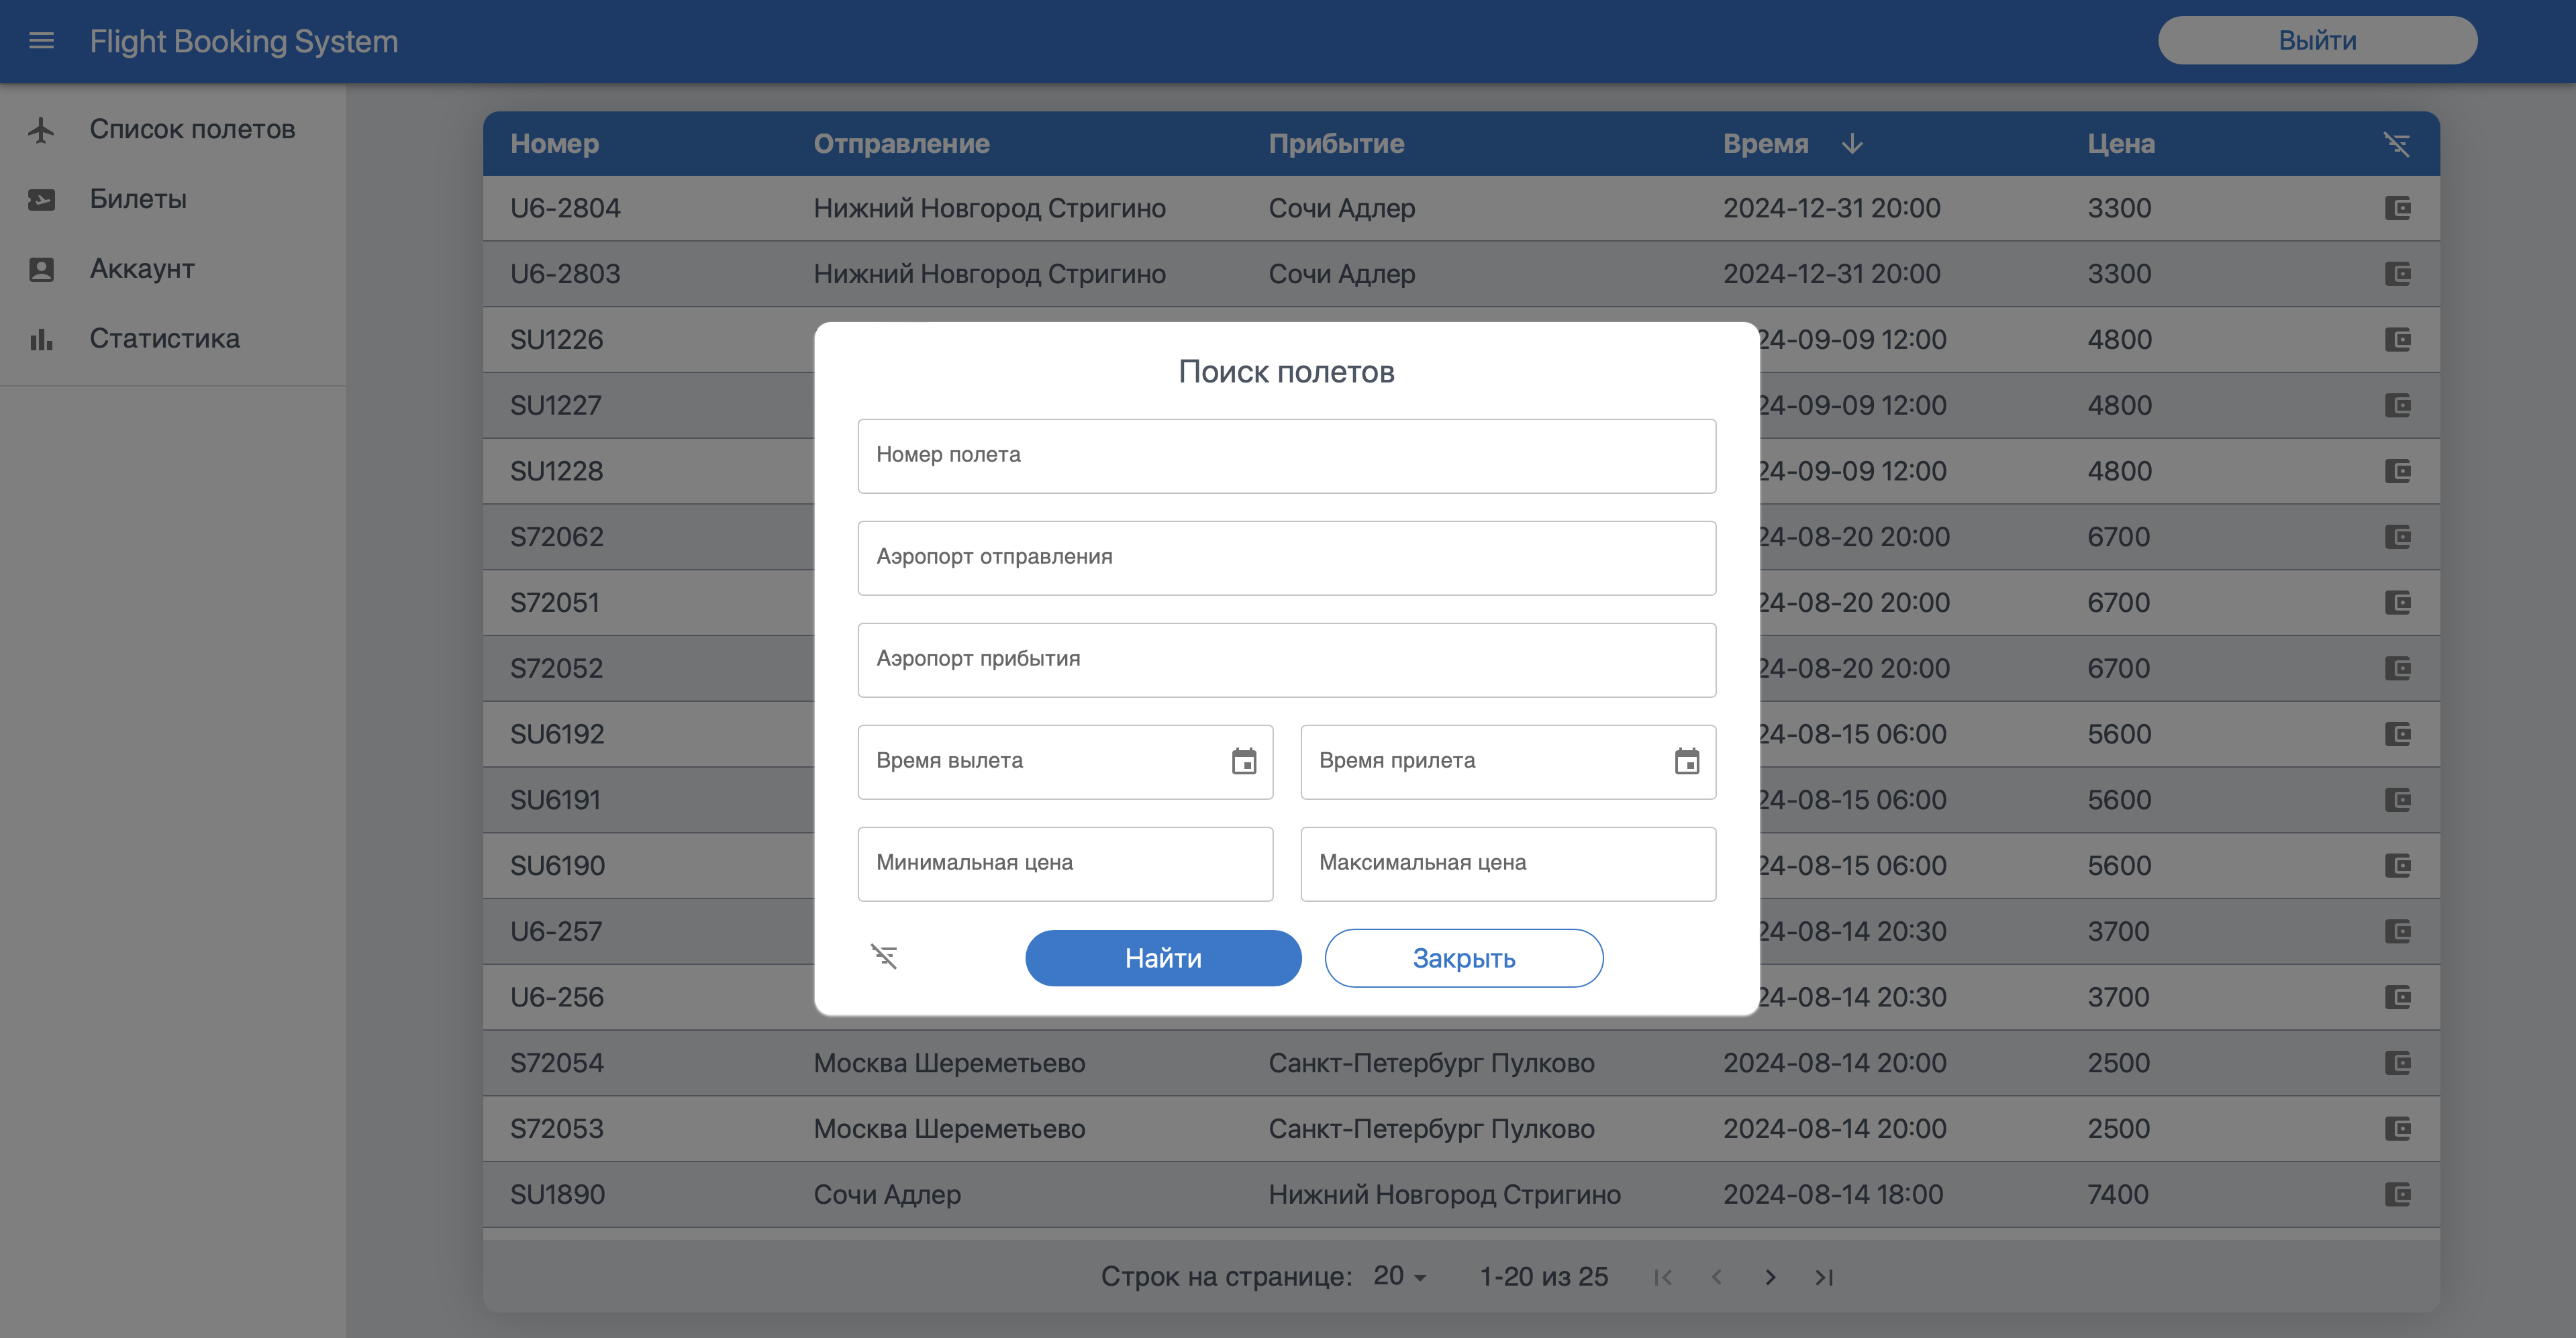
\includegraphics[scale = 0.25]{../img/pages/page-03.png}}
		\caption{Страница с полетами (пример сортировки и фильтрации)}
		\label{fig:page-03}
	\end{center}
\end{figure}

\begin{figure}[H]
	\begin{center}
		{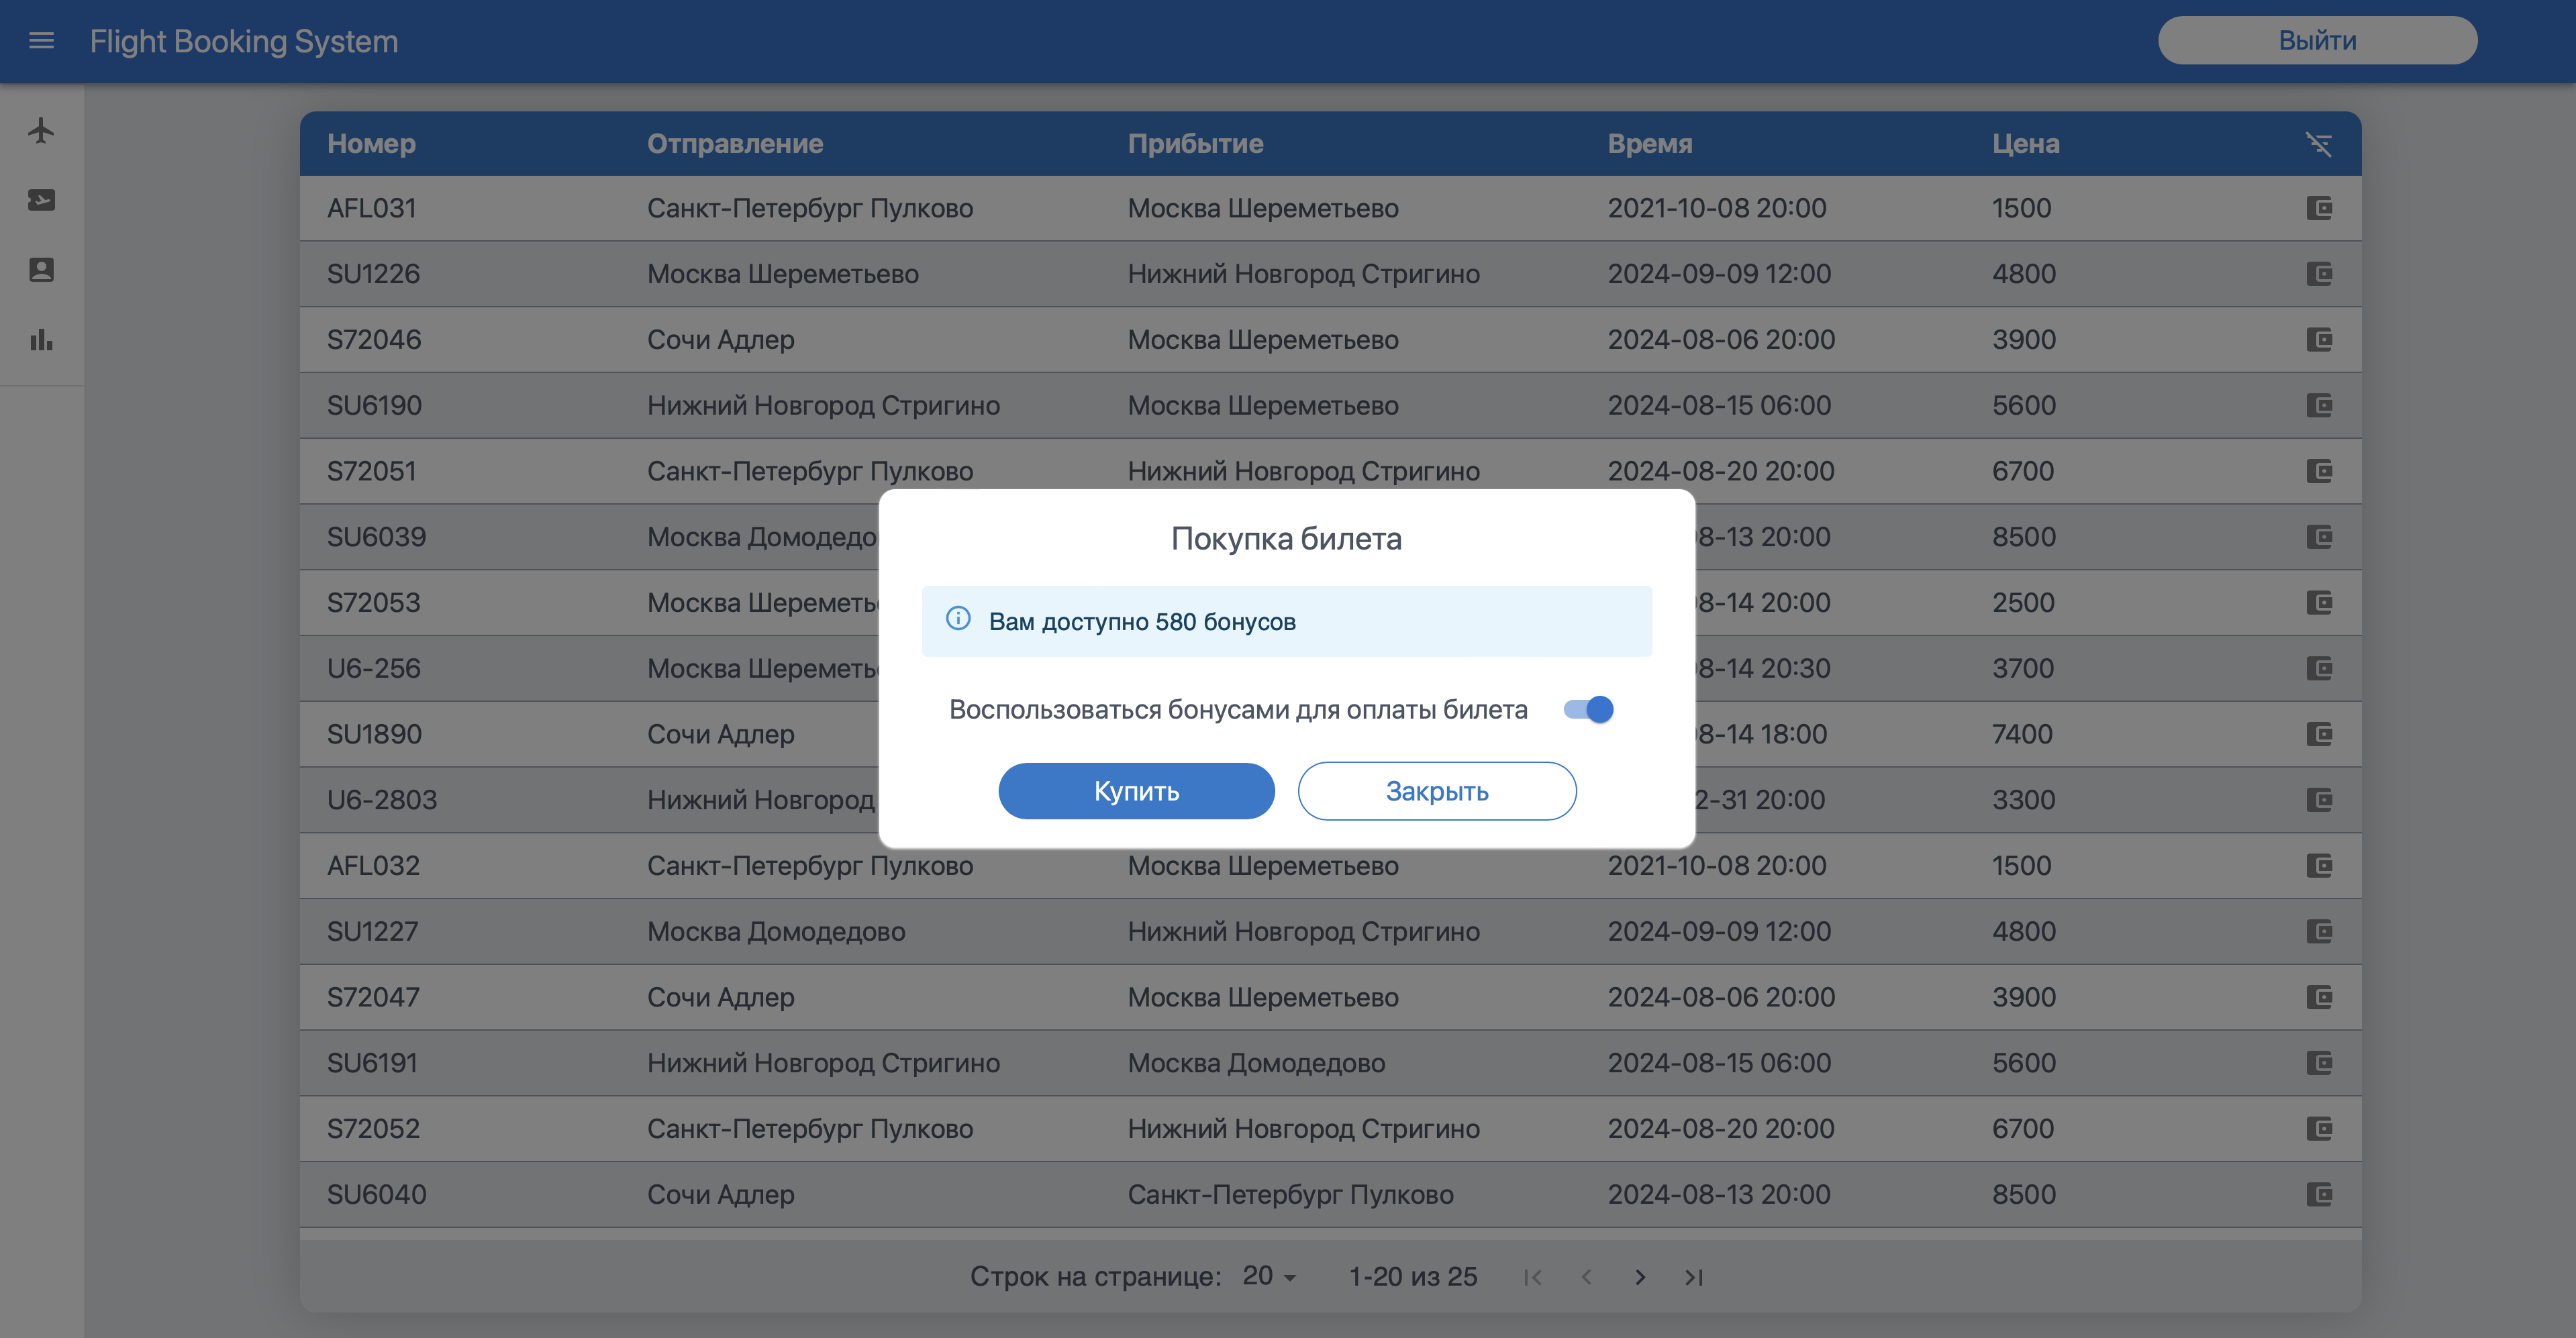
\includegraphics[scale = 0.25]{../img/pages/page-04.png}}
		\caption{Страница с полетами (пример покупки билета)}
		\label{fig:page-04}
	\end{center}
\end{figure}

\begin{figure}[H]
	\begin{center}
		{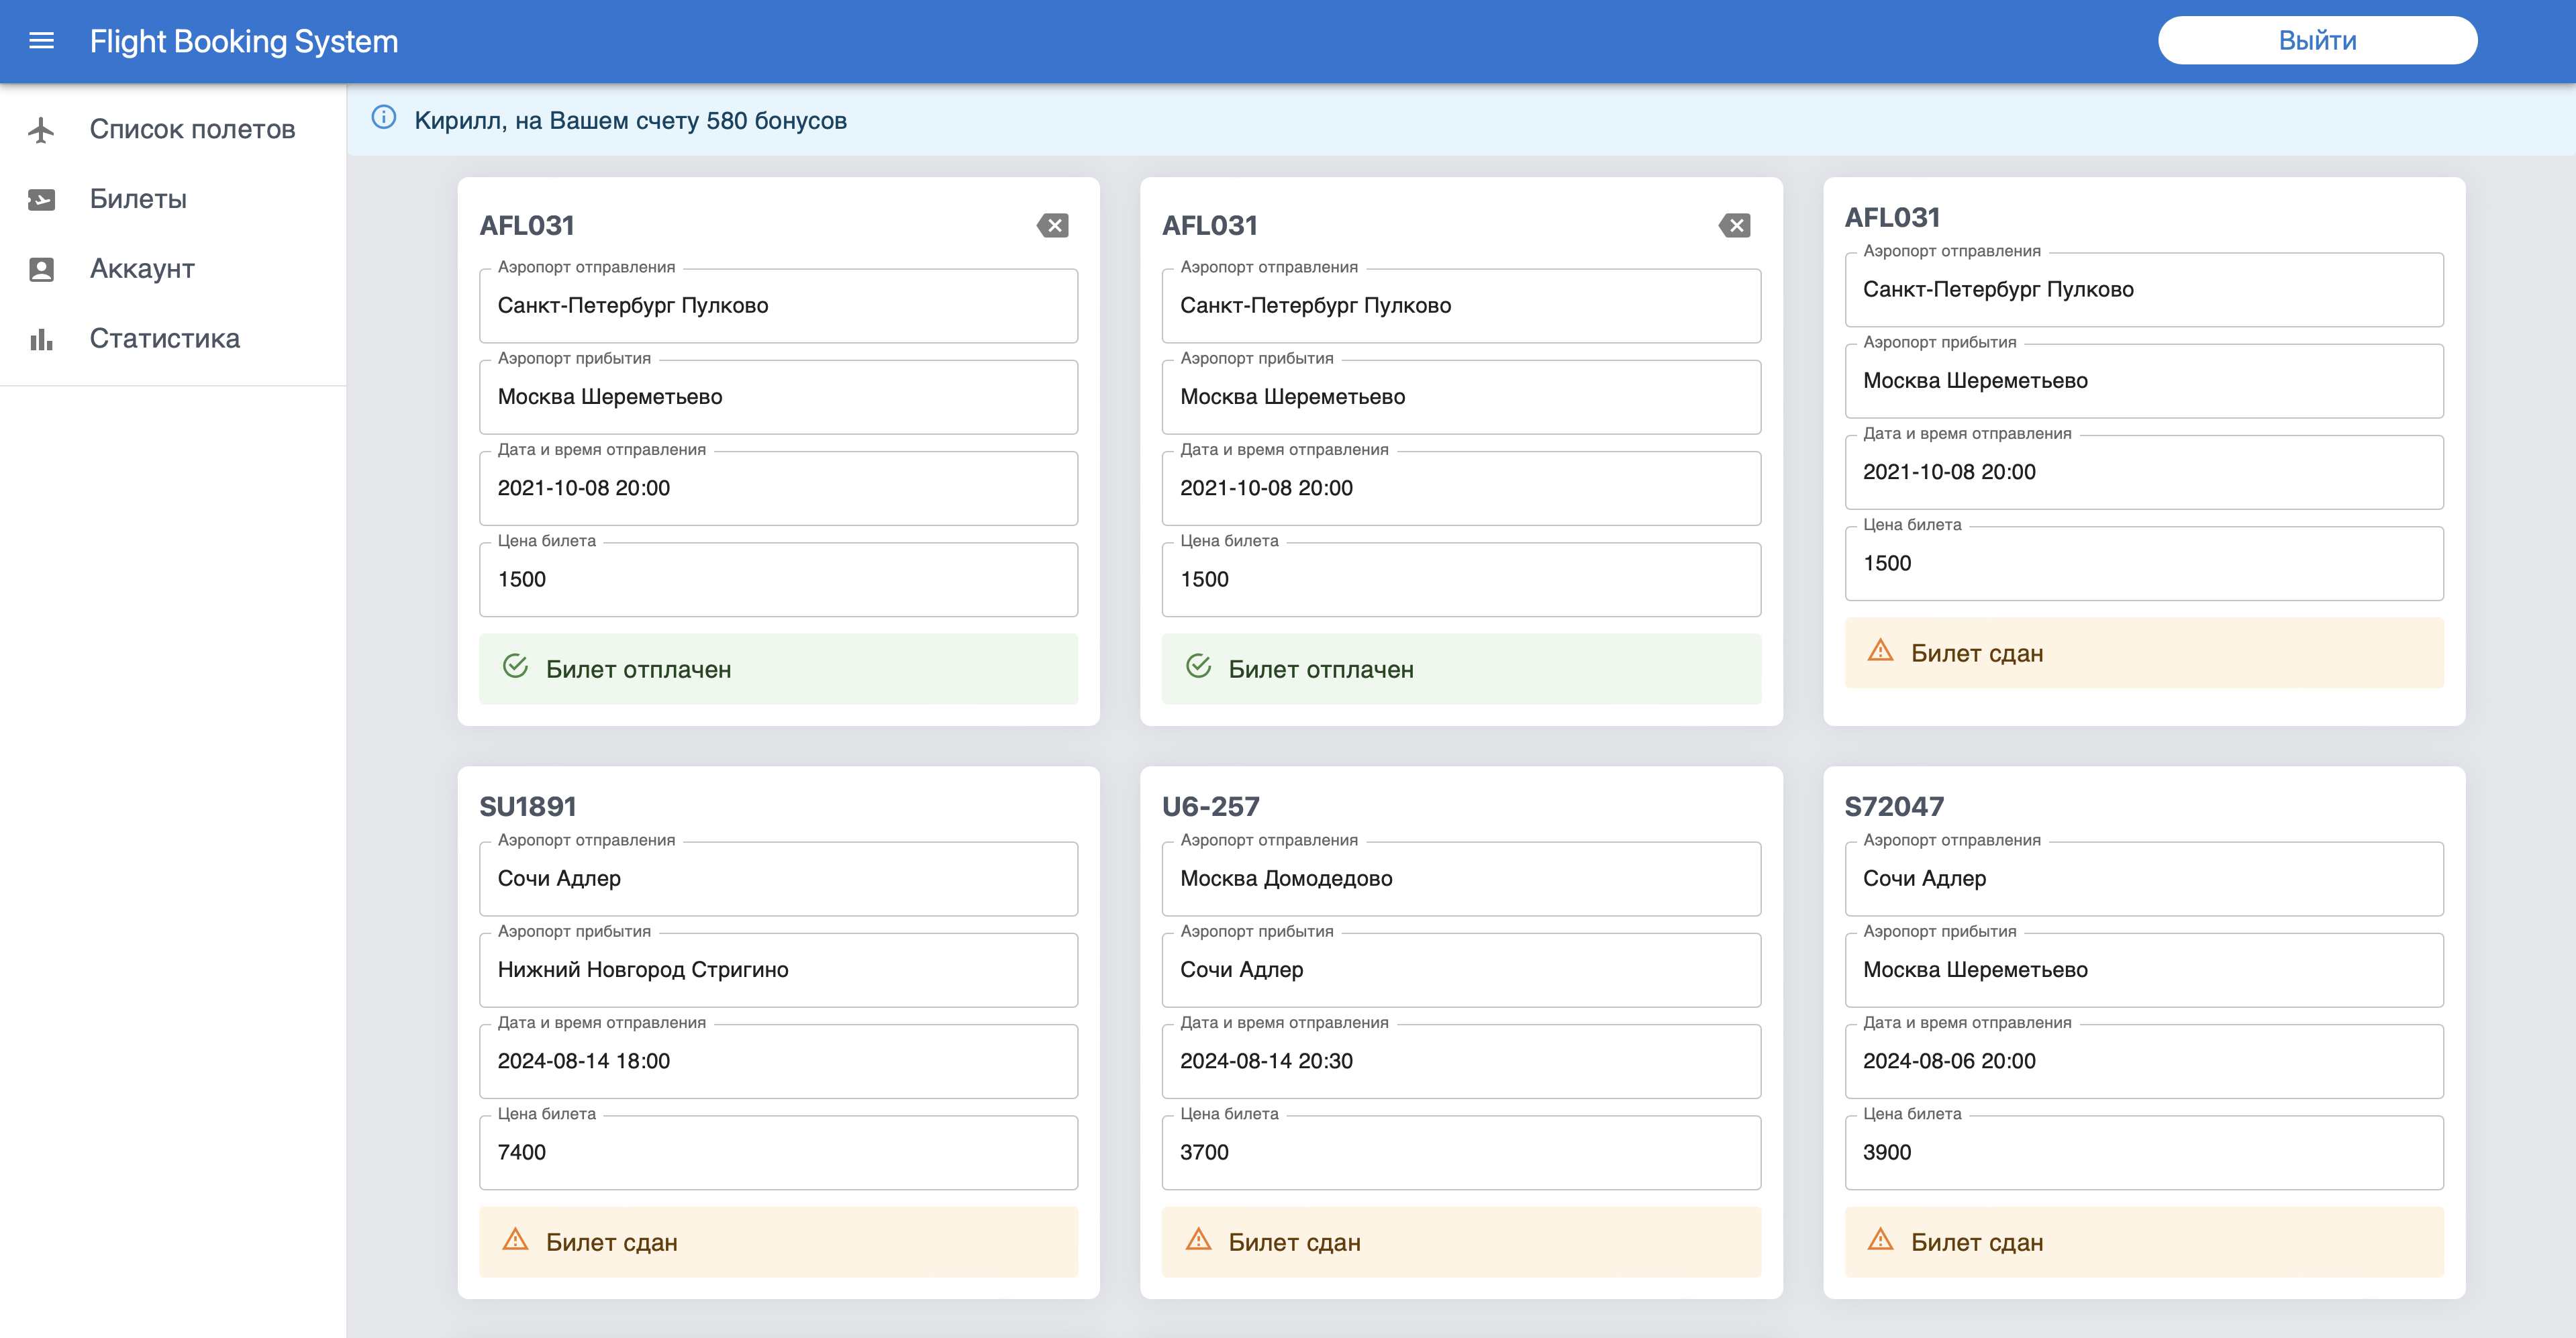
\includegraphics[scale = 0.25]{../img/pages/page-05.png}}
		\caption{Страница с купленными и сданными билетами}
		\label{fig:page-05}
	\end{center}
\end{figure}

\begin{figure}[H]
	\begin{center}
		{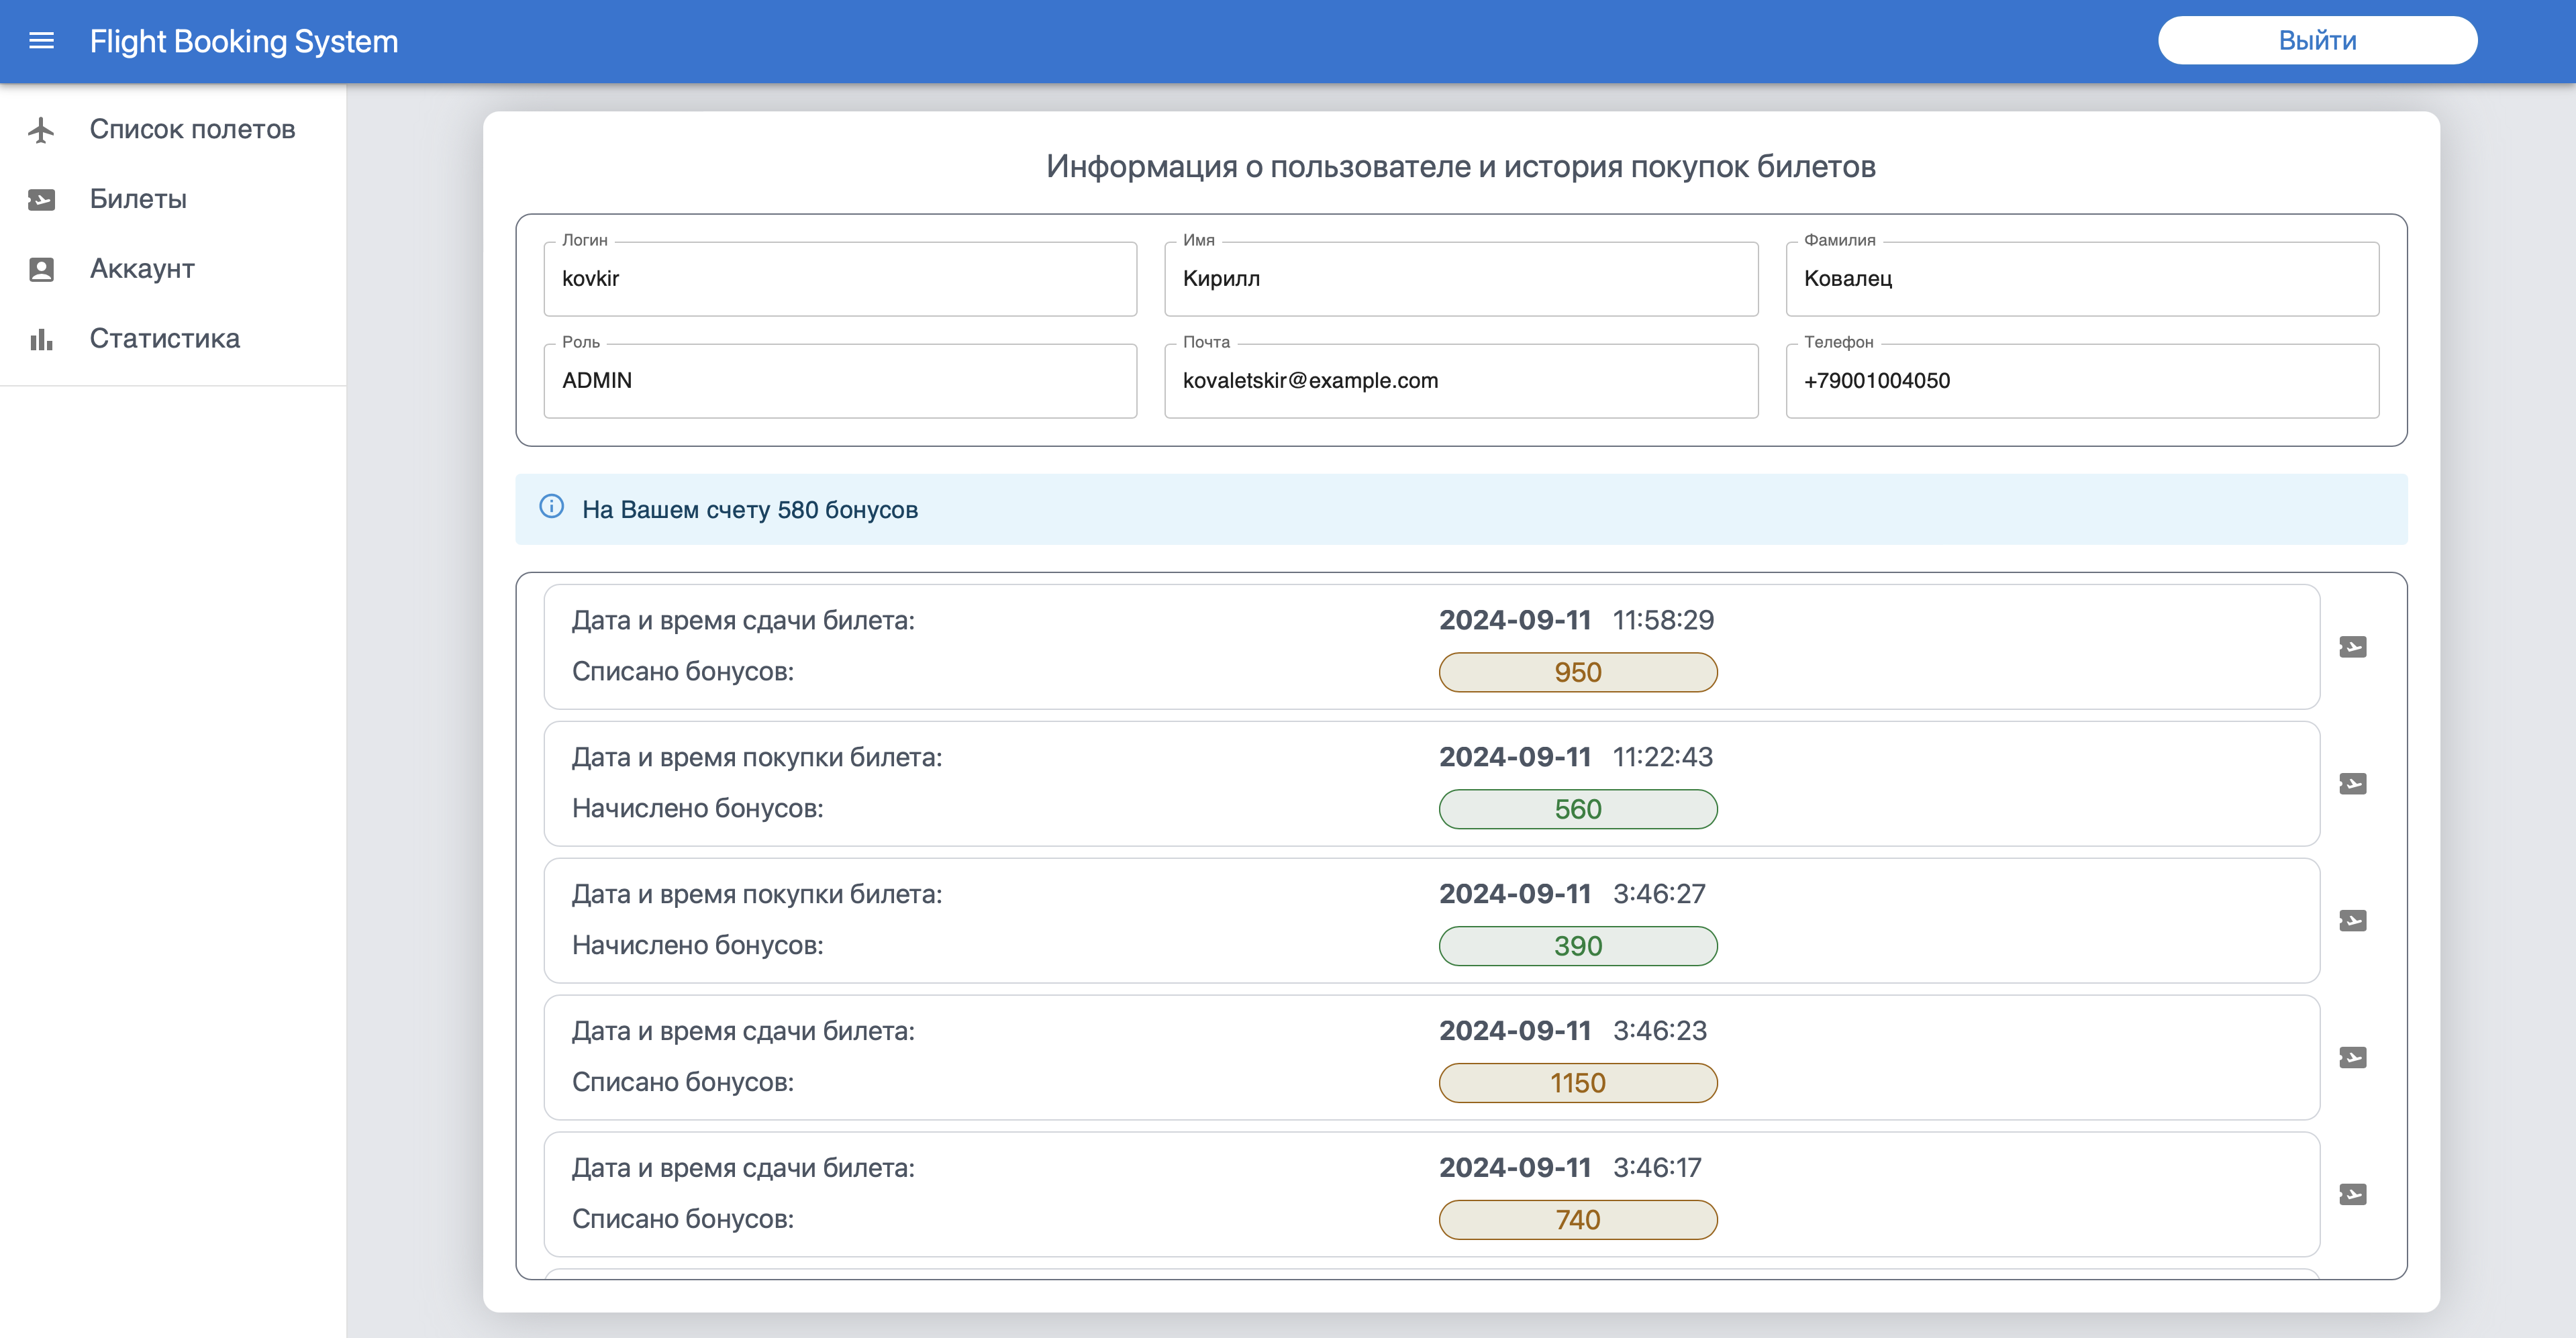
\includegraphics[scale = 0.25]{../img/pages/page-06.png}}
		\caption{Страница с информацией о пользователе и историей покупок}
		\label{fig:page-06}
	\end{center}
\end{figure}

\begin{figure}[H]
	\begin{center}
		{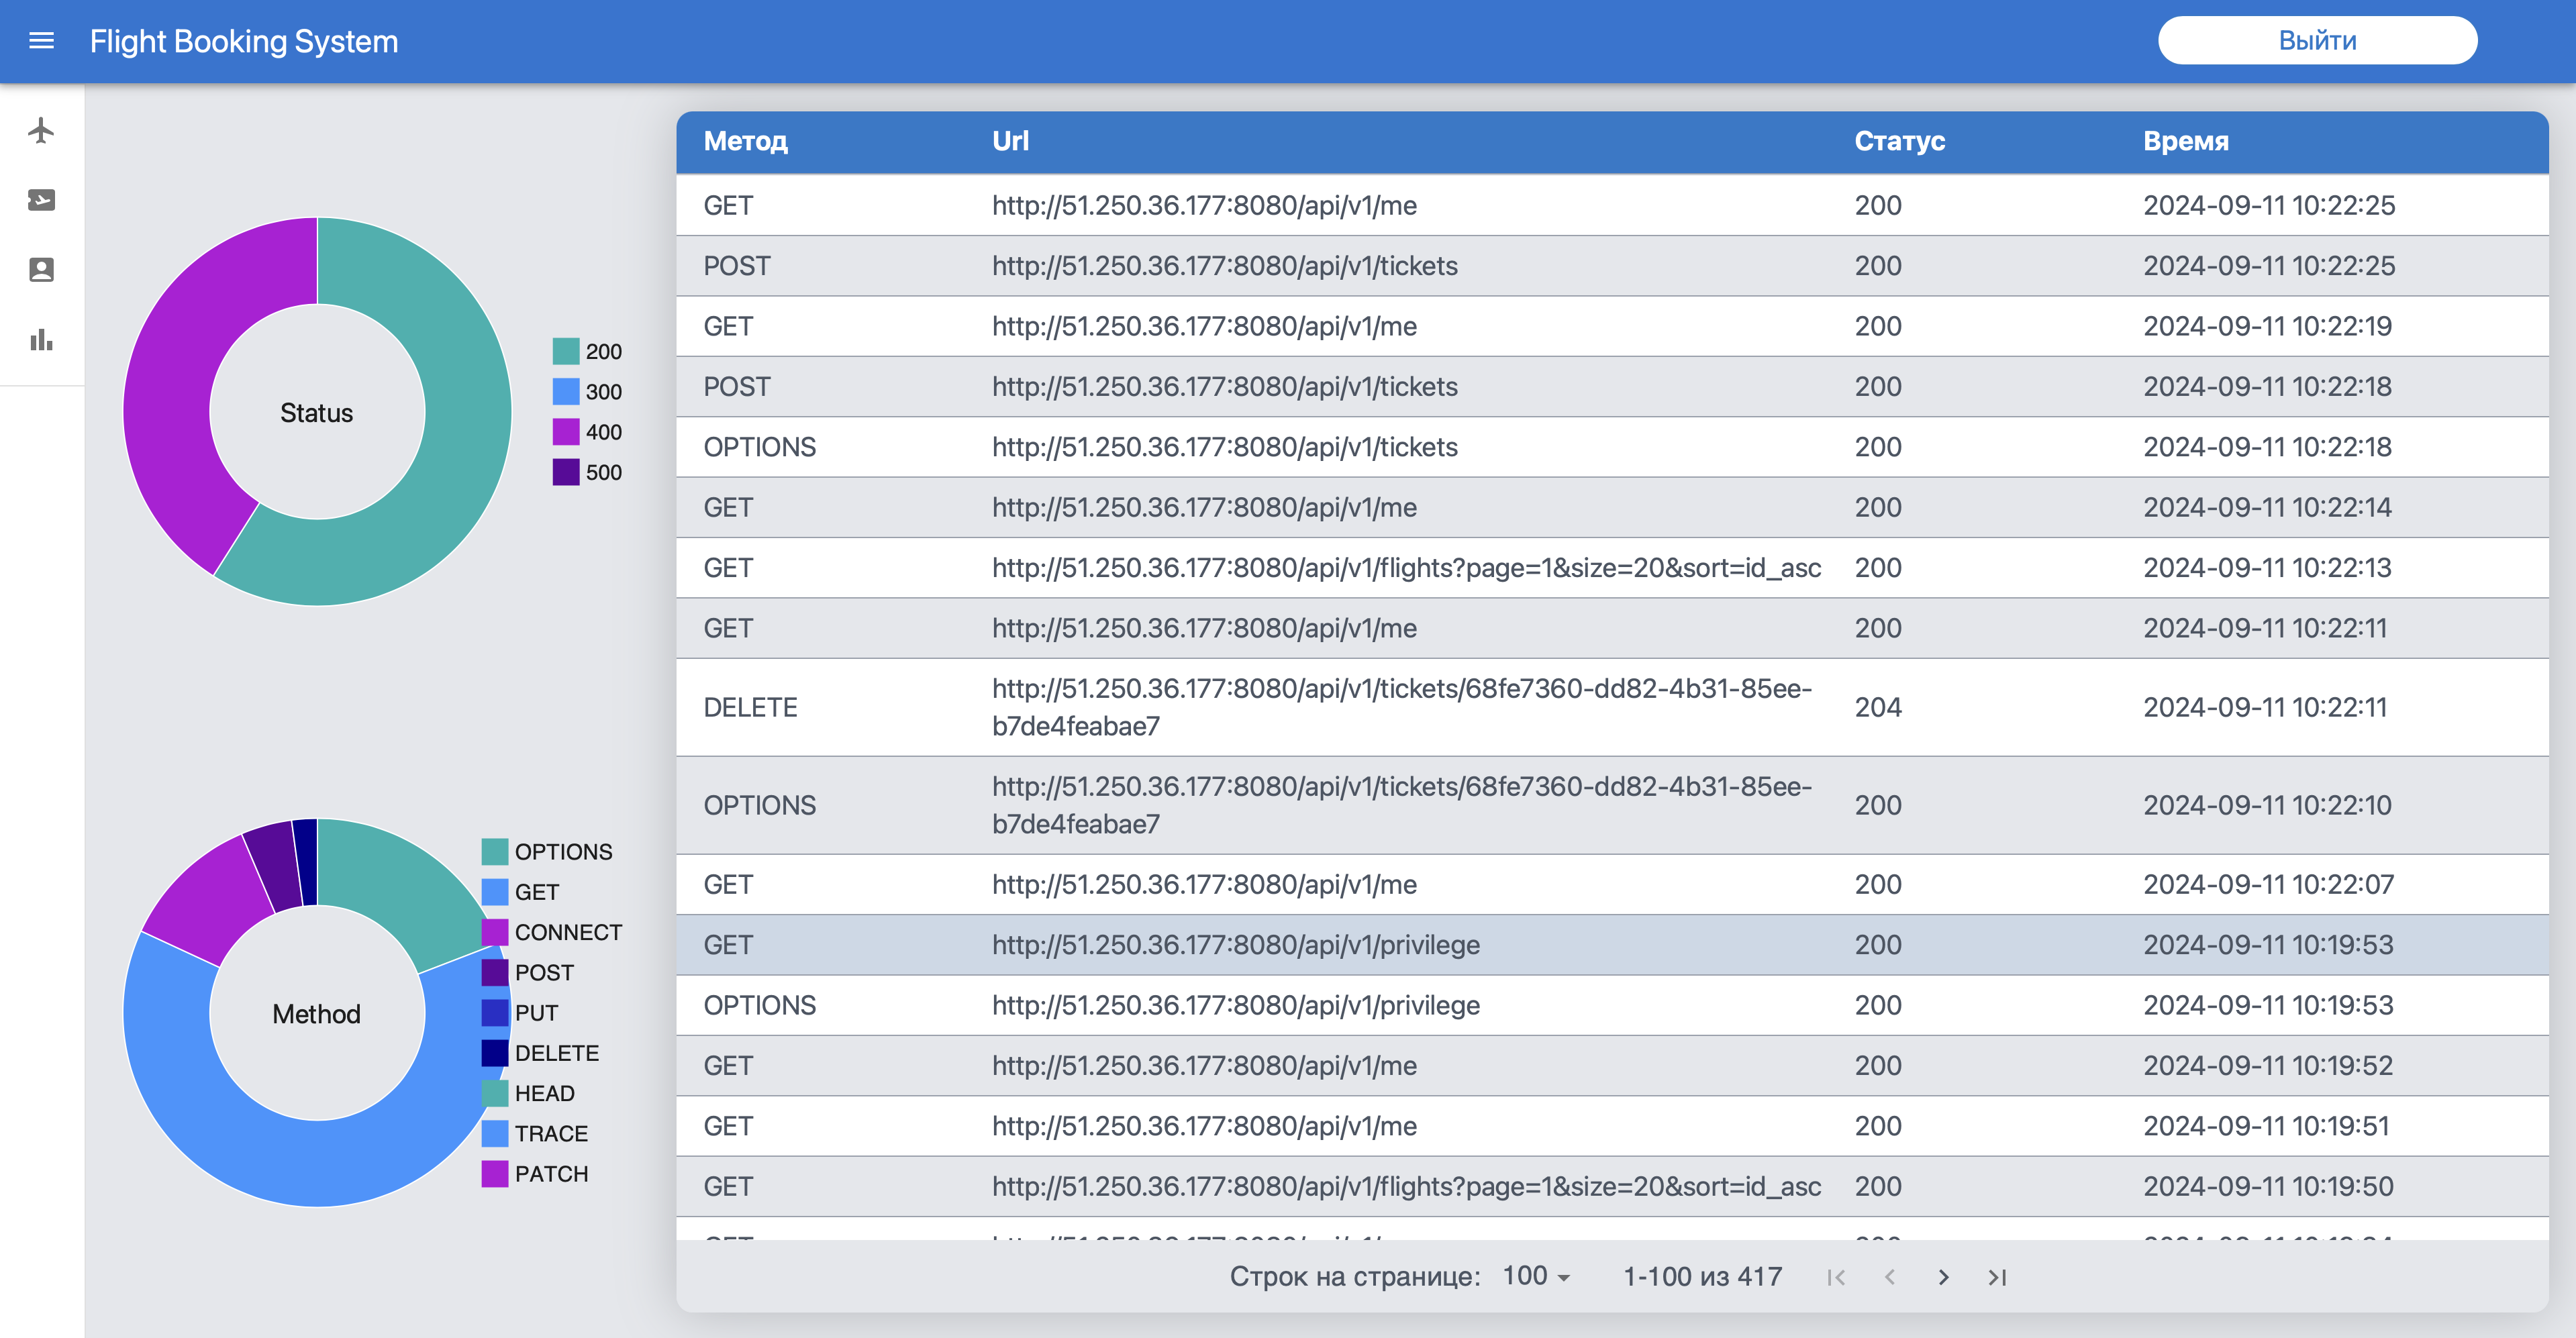
\includegraphics[scale = 0.25]{../img/pages/page-07.png}}
		\caption{Страница со статистикой}
		\label{fig:page-07}
	\end{center}
\end{figure}
